% Binary-level verification of the XRP Ledger close-time computation.
% Build:  tectonic paper/xrpl-close-time.tex
\documentclass[11pt,a4paper]{article}

\usepackage{fontspec}
\usepackage[a4paper,margin=25mm]{geometry}
\usepackage{amsmath,amssymb,amsthm}
\usepackage{booktabs}
\usepackage{tabularx}
\usepackage{array}
\usepackage{xcolor}
\usepackage{upquote}
\usepackage{listings}
\usepackage{tikz}
\usetikzlibrary{arrows.meta}
\usepackage{enumitem}
\usepackage[font=small,labelfont=bf,justification=raggedright,singlelinecheck=false]{caption}
\usepackage{microtype}
\usepackage[colorlinks=true,linkcolor=link,citecolor=link,urlcolor=link]{hyperref}
\hypersetup{
  pdftitle={Binary-Level Verification of the XRP Ledger Close-Time Computation},
  pdfauthor={Phil Kwok}}

\definecolor{link}{HTML}{1F3A6E}
\definecolor{kw}{HTML}{1F3A6E}
\definecolor{cmt}{HTML}{5B6470}
\definecolor{rule}{HTML}{9AA3AE}
\definecolor{trusted}{HTML}{E4E8EE}

\setlist{itemsep=2pt,topsep=4pt,leftmargin=1.6em}
\frenchspacing
\emergencystretch=1.5em

\lstdefinelanguage{Rocq}{
  morekeywords={Theorem,Lemma,Definition,Example,Proof,Qed,Module,End,forall,
    exists,fun,if,then,else,let,in},
  sensitive=true,
  morecomment=[s]{(*}{*)}}
\lstdefinestyle{code}{
  basicstyle=\ttfamily\small,
  columns=fullflexible,
  keepspaces=true,
  breaklines=true,
  breakatwhitespace=true,
  showstringspaces=false,
  frame=lines,
  rulecolor=\color{rule},
  framesep=5pt,
  aboveskip=10pt,
  belowskip=6pt,
  keywordstyle=\color{kw},
  commentstyle=\color{cmt}\itshape,
  captionpos=b}
\lstset{style=code}

\newcommand{\code}[1]{\texttt{\upshape\detokenize{#1}}}
\newcommand{\fpath}[1]{\nolinkurl{#1}}
\newcommand{\rnd}{\operatorname{round}}
\newcommand{\eff}{\operatorname{eff}}
\newcommand{\sx}{\operatorname{sx}_{32}}
\newcommand{\W}{2^{32}}

\newtheorem{theorem}{Theorem}
\theoremstyle{definition}
\newtheorem{definition}{Definition}

\title{\textbf{Binary-Level Verification of the\\
XRP Ledger Close-Time Computation}\\[8pt]
\large A machine-checked proof in Rocq over compiled RISC-V code}
\author{Phil Kwok\\[4pt]
\normalsize\textit{BA, MA (Scholar) --- Cambridge University}\\[2pt]
\normalsize EasyA}
\date{23 November 2026}

\begin{document}
\maketitle

\begin{abstract}
\noindent Anthropic and Theorem recently reported machine-checked proofs,
produced by a language model, that 239 fuzzing entry points in open-source
libraries cannot crash; the proofs are stated over the compiled RISC-V
binaries~\cite{anthropic}. We apply the same method and the same published
model of a Linux process~\cite{lps} to a small part of the XRP Ledger server,
\texttt{xrpld}: the function that converts the close time agreed by
validators into the close time recorded in a ledger header. Three results
are proved in Rocq~\cite{rocq}. The nine machine instructions compiled from
the function compute a 32-bit integer specification for every input. The
specification has the properties on which consensus depends, namely that a
ledger closes strictly after its predecessor and on a resolution boundary
close to the agreed time. Finally, an 87-instruction test program built
around the function exits with status~0 on every valid launch and never
executes its trap instruction; this theorem is an instance of the statement
published with the model. The proofs depend on no axioms other than Rocq's
primitive integers, strings and arrays. The scope is one function compiled
for one target, and the development has not yet been independently reviewed.
We describe the trusted computing base and the limitations of the result,
and outline what applying the method to more of \texttt{xrpld} would
require.
\end{abstract}

\section{Introduction}

Most software is validated by testing. A unit test exercises a single input
and a fuzzer exercises many, but both sample the input space. A formal proof
establishes a property for all inputs by an argument that a small trusted
program, the proof checker, verifies mechanically. Constructing such proofs
has historically been costly, and end-to-end examples such as the seL4
kernel~\cite{sel4} and the CompCert compiler~\cite{compcert} remain rare.

In October 2026 Anthropic and Theorem reported a sharp reduction in that
cost~\cite{anthropic}. A language model produced proofs that 239 fuzzing
entry points across 123 open-source libraries do not crash on any input of
up to 64\,MB. The proofs concern the compiled RISC-V binaries, not the
source code, and total about 180 million lines of Rocq; a typical proof is
about 600,000 lines for a binary with a median size of 18,000 instructions.
The method starts from an existing fuzz target, reads it as a claim about
every input, and proves that claim of the binary.

Machine-checked proof on this scale is no longer confined to software. On
20~November 2026 Alp\"oge announced a proof of the Riemann Hypothesis,
developed with Claude and released as a Lean library of 17 million lines
with no accompanying paper~\cite{alpoge}. The Lean and Mathlib communities
have since reported that both the formal statement and the proof
check~\cite{leanrh}. There, as here, the proof itself does not have to be
read, and the part that calls for human scrutiny is the statement that was
proved.

Formal verification of the XRP Ledger is already in progress at the level of
protocol models. Ripple and Common Prefix published a specification of the
Payment Engine in December 2025 and announced plans to verify it and the
consensus protocol~\cite{ripplex}; in 2026 Common Prefix began modelling the
Lending Protocol in Lean~4~\cite{cryptoslate}. Ripple describes this as ``an
act of modelling and abstraction, not translation''~\cite{ripplex}. Agreement
between the model and the C++ implementation is checked by differential
testing~\cite{cryptoslate}, and the compiler's translation of the C++ is, as
far as the public descriptions indicate, out of scope.

This report applies the method of~\cite{anthropic} to code from
\texttt{xrpld}~\cite{rippled}. The target is the ledger close-time
computation in \code{LedgerTiming.h}, which is small, self-contained and
used by consensus, and which we take from the upstream repository without
modification. We prove the following.

\begin{enumerate}
\item The nine RISC-V instructions compiled from \code{effCloseTime} return
  the value of an integer specification for all
  $\W \cdot (\W-1) \cdot \W \approx 7.9 \times 10^{28}$ combinations of
  32-bit inputs (Theorem~\ref{thm:code}).
\item The specification guarantees that a ledger closes strictly after its
  predecessor, and either one second after it or on a resolution boundary
  within half a resolution of the agreed time
  (Theorems~\ref{thm:after}--\ref{thm:nearest}).
\item An 87-instruction program that decodes an input, calls the function
  and checks its result terminates with \code{exit(0)} on every valid launch
  (Theorem~\ref{thm:halts}). This is an instance of \code{halts_allowed_T},
  the statement published with the model and used for the proofs
  in~\cite{anthropic}.
\end{enumerate}

\noindent The proof effort also exposed an overflow in our own test harness,
and the theorems identify the inputs for which the 32-bit representation of
time affects the result (Section~\ref{sec:findings}). The proof scripts
comprise 1,844 lines of Rocq.

The result is limited to nine instructions of one function, compiled for
RISC-V by one compiler at one optimisation level. It does not establish the
correctness of \texttt{xrpld} or of its release binaries, and the test and
its properties are ours, not the maintainers'. Section~\ref{sec:limits}
discusses these limitations.

\section{Background}

\subsection{Close time in the XRP Ledger}

Every ledger header records a close time, a count of seconds since
1~January 2000 UTC held in an unsigned 32-bit integer (\code{NetClock} in
\code{xrpl/basics/chrono.h}). Because validators' clocks differ, consensus
does not attempt to agree on an exact second. Validators agree instead on a
time rounded to a \emph{resolution}, one of the six values 10, 20, 30, 60,
90 and 120 seconds listed in \code{kLedgerPossibleTimeResolutions}. The
protocol and its analysis are described in~\cite{rpca,chase}.

When a round agrees on a close time, \texttt{xrpld} computes the value
stored in the new ledger by calling \code{effCloseTime} (in
\code{RCLConsensus.cpp}). Listing~\ref{lst:cpp} shows this function and the
rounding function it calls. Both are header templates, instantiated at the
call site with the 32-bit types of \code{NetClock}.

\begin{lstlisting}[language=C++,float=t,label=lst:cpp,
  caption={The code under proof, from \texttt{include/xrpl/ledger/LedgerTiming.h}
  of \texttt{xrpld} at commit \texttt{82217fbd} (ISC licence, copyright the XRP
  Ledger developers). Template headers and \texttt{using} declarations are
  omitted, parameter types are abbreviated and one line is wrapped.}]
roundCloseTime(time_point closeTime, duration closeResolution)
{
    if (closeTime == time_point{})
        return closeTime;

    closeTime += (closeResolution / 2);
    return closeTime - (closeTime.time_since_epoch() % closeResolution);
}

effCloseTime(time_point closeTime, duration resolution, time_point priorCloseTime)
{
    if (closeTime == time_point{})
        return closeTime;

    return std::max<time_point>(
        roundCloseTime(closeTime, resolution), (priorCloseTime + 1s));
}
\end{lstlisting}

A close time of zero denotes the absence of a close time and is returned
unchanged. Any other value is rounded to the nearest multiple of the
resolution and then raised, if necessary, to one second after the previous
ledger's close time. The existing unit tests for the two functions consist
of 13 assertions on example values
(\fpath{src/tests/libxrpl/consensus/LedgerTiming.cpp}), five of which
concern \code{effCloseTime}.

\subsection{Binary-level statements from tests}

The method of~\cite{anthropic} starts from a test program that signals
failure by crashing. The claim that no input makes the test fail then
becomes the claim that the process exits normally on every input, which is a
statement about the compiled binary and the machine that runs it.

Theorem's \emph{Linux process semantics} (LPS)~\cite{lps} makes this
statement precise. LPS is a Rocq model of a single process on Linux v6.18.46
for \texttt{riscv64}. It covers the RV64GC instruction set~\cite{riscv}, the
initial placement of the stack, arguments and environment, and the
system-call interface. Listing~\ref{lst:halts} shows its statement
\code{halts_allowed_T}. An \emph{image} consists of the contents of a
binary's loadable segments, its entry address and its program headers. The
statement asserts that for every launch the model admits
(\code{valid_entry}, which covers the position of the stack and the random
bytes supplied by the kernel, among other things) and every admissible input
(\code{valid_input}, the argument list and the environment), every execution
exits with a status in the list~$S$.

\begin{lstlisting}[language=Rocq,float=t,label=lst:halts,
  caption={The statement instantiated by Theorem~\ref{thm:halts}, from LPS
  (\texttt{EquivalenceDefinition/HaltsAllowed.v}).}]
Definition halts_allowed_T (S : list word) (img : Image) : Prop :=
  forall en inp,
    valid_entry img en inp ->
    valid_input inp ->
    must_exit_in S img source_alloc_limit en inp.
\end{lstlisting}

A proof of such a statement is checked by the Rocq kernel and does not
itself need to be read or trusted. The trusted base is the kernel, the model
and the statement; Section~\ref{sec:trust} gives details.

\section{The verified binary}
\label{sec:binary}

\begin{figure}[t]
\centering
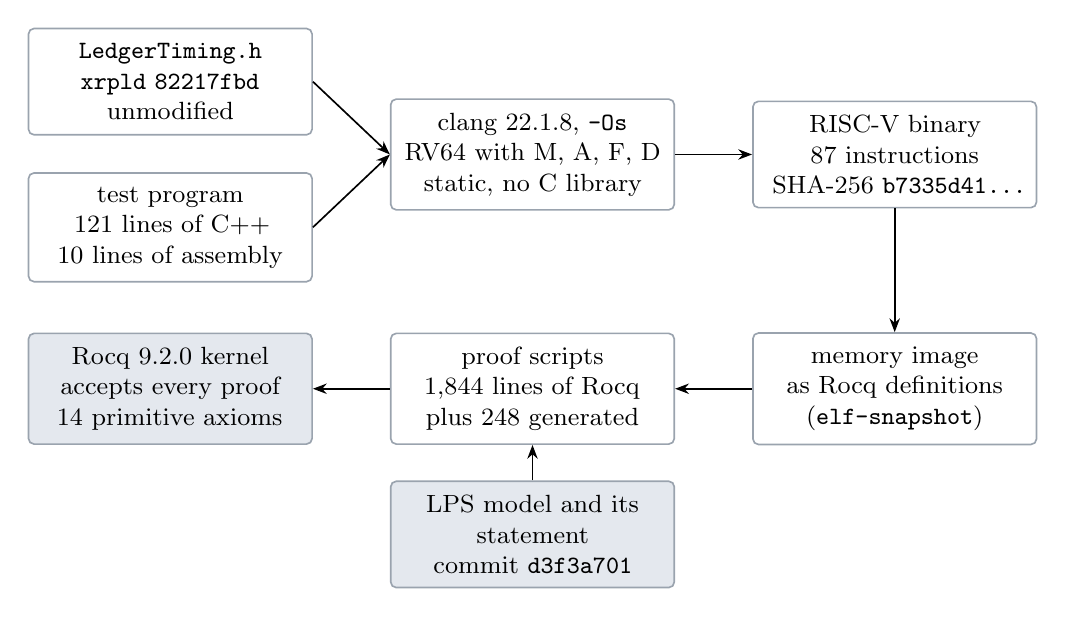
\begin{tikzpicture}[
  box/.style={draw=rule, line width=0.6pt, rounded corners=2pt, align=center,
    font=\small, inner sep=5pt, text width=3.25cm, minimum height=1.35cm},
  arr/.style={-{Stealth[length=5pt]}, line width=0.6pt}]
\node[box] (src) at (0,0)
  {\texttt{LedgerTiming.h}\\ \texttt{xrpld} \texttt{82217fbd}\\ unmodified};
\node[box] (har) at (0,-1.85)
  {test program\\ 121 lines of C++\\ 10 lines of assembly};
\node[box] (cc) at (4.6,-0.925)
  {clang 22.1.8, \texttt{-Os}\\ RV64 with M, A, F, D\\ static, no C library};
\node[box] (bin) at (9.2,-0.925)
  {RISC-V binary\\ 87 instructions\\ SHA-256 \texttt{b7335d41\ldots}};
\node[box] (img) at (9.2,-3.9)
  {memory image\\ as Rocq definitions\\ (\texttt{elf-snapshot})};
\node[box] (prf) at (4.6,-3.9)
  {proof scripts\\ 1,844 lines of Rocq\\ plus 248 generated};
\node[box, fill=trusted] (ker) at (0,-3.9)
  {Rocq 9.2.0 kernel\\ accepts every proof\\ 14 primitive axioms};
\node[box, fill=trusted] (lps) at (4.6,-5.75)
  {LPS model and its\\ statement\\ commit \texttt{d3f3a701}};
\draw[arr] (src.east) -- (cc.west);
\draw[arr] (har.east) -- (cc.west);
\draw[arr] (cc) -- (bin);
\draw[arr] (bin) -- (img);
\draw[arr] (img) -- (prf);
\draw[arr] (prf) -- (ker);
\draw[arr] (lps) -- (prf);
\end{tikzpicture}
\caption{From the upstream source to the checked theorems. The shaded
components, and the step that converts the binary into Rocq definitions,
form the trusted base. The compiler and the proof scripts are outside it.}
\label{fig:pipeline}
\end{figure}

\paragraph{Test program.} The file \fpath{harness/close_time_harness.cpp}
includes the two upstream headers unmodified and wraps \code{effCloseTime},
instantiated with the types of \code{NetClock} as in consensus, in a single
out-of-line function. Its \code{main} decodes one argument into a close
time~$c$, a previous close time~$p$ and an index into the table of
resolutions, calls the function, and executes a trap instruction if any of
the following fails:

\begin{enumerate}
\item if $c = 0$, the result is $0$;
\item otherwise the result is strictly greater than $p$;
\item the result is $p + 1$, or it is a multiple of the resolution within
  half a resolution of $c$.
\end{enumerate}

\noindent The argument has 17 characters, and only the low four bits of each
are used: eight characters encode $c$, eight encode $p$ and one encodes the
index. This encoding represents every 32-bit value without a zero byte,
which a C string cannot contain. Launches with a different number of
arguments, a shorter argument, an index above~5 or a time beyond the horizon
$H = \W - 61$ exit with status~0 without running the checks. $H$ is the last
second for which no step of the arithmetic can wrap for any legal
resolution, and corresponds to 06:27:15 UTC on 7~February 2136.

\paragraph{Build.} The binary is freestanding and uses no C library. A
six-instruction entry point reads \code{argc} and \code{argv} from the
initial stack, calls \code{main} and passes the result to the \code{exit}
system call. We compile with clang~22.1.8, as distributed with zig~0.17.1,
for \texttt{riscv64} with the M, A, F and D extensions at \code{-Os}, and
link statically, without debug information, which would record the build
directory. The build is reproducible: builds in three directories, from two
separately fetched copies of the sources, produce identical files. The
resulting binary contains 87
instructions, of which six belong to the entry point, nine to the function
under proof and 72 to \code{main}. It has two loadable segments: read-only
data at \code{0x10000}, which holds the table of resolutions, and code at
\code{0x11000}. Its SHA-256 digest is\\
\code{b7335d41d947f9aba48913556f7b42dd2926a9b50041ec649b9ee05f5825b257}.

\paragraph{Compiled function.} Table~\ref{tab:asm} lists the function as
compiled. The compiler has inlined the rounding function, leaving
straight-line arithmetic with two branches.

\begin{table}[t]
\centering
\small
\begin{tabular}{@{}llll@{}}
\toprule
Address & Word & Instruction & Effect \\
\midrule
\code{11018} & \code{02050063} & \code{beq   a0, zero, 11038} & close time is 0: return it \\
\code{1101c} & \code{0015d69b} & \code{srliw a3, a1, 1}       & half the resolution \\
\code{11020} & \code{00a68533} & \code{add   a0, a3, a0}      & close time plus half the resolution \\
\code{11024} & \code{02b575bb} & \code{remuw a1, a0, a1}      & remainder modulo the resolution \\
\code{11028} & \code{40b5053b} & \code{subw  a0, a0, a1}      & the rounded close time \\
\code{1102c} & \code{0016061b} & \code{addiw a2, a2, 1}       & previous close time plus 1 \\
\code{11030} & \code{00a66463} & \code{bltu  a2, a0, 11038}   & if that is smaller, keep the rounded time \\
\code{11034} & \code{00060513} & \code{addi  a0, a2, 0}       & otherwise take previous close plus 1 \\
\code{11038} & \code{00008067} & \code{jalr  zero, 0(ra)}     & return \\
\bottomrule
\end{tabular}
\caption{The function under proof as it appears in the binary. On entry
\texttt{a0}, \texttt{a1} and \texttt{a2} hold the close time, the resolution
and the previous close time.}
\label{tab:asm}
\end{table}

\paragraph{Embedding in Rocq.} The \code{elf-snapshot} tool distributed with
LPS writes the segments of the binary as Rocq definitions. For each of the
87 instruction addresses a script then generates a lemma stating the 32-bit
word that the model fetches at that address and, for every instruction other
than the system call, a second lemma stating the instruction that the
model's decoder assigns to that word. Rocq proves these lemmas by
computation, so the generator is not trusted.

\section{Specification}
\label{sec:spec}

The specification is stated over the unbounded integers and reproduces the
wrap-around at $\W$ of 32-bit arithmetic. Its definitions occupy the first
42 lines of \code{CloseTimeSpec.v}. Since Theorem~\ref{thm:code} is only as meaningful
as these definitions, they are the part of the development that a reviewer
should read first.

\begin{definition}[Close-time rule]
For integers $c$ (close time), $r$ (resolution) and $p$ (previous close
time), let $x = (c + \lfloor r/2 \rfloor) \bmod \W$ and
\begin{align*}
\rnd(c, r) &=
  \begin{cases}
    0 & \text{if } c = 0,\\
    (x - (x \bmod r)) \bmod \W & \text{otherwise;}
  \end{cases}\\[4pt]
\eff(c, r, p) &=
  \begin{cases}
    0 & \text{if } c = 0,\\
    \max\bigl(\rnd(c, r),\ (p + 1) \bmod \W\bigr) & \text{otherwise.}
  \end{cases}
\end{align*}
\end{definition}

\noindent Let $R = \{10, 20, 30, 60, 90, 120\}$ denote the set of legal
resolutions and $H = \W - 61$ the horizon. The following theorems are proved
in Rocq from the definition alone; they involve no machine code and depend
on no axioms.

\begin{theorem}[\code{eff_after_prior}]\label{thm:after}
If $0 < c < \W$ and $0 \le p < \W - 1$, then $p < \eff(c, r, p)$ for every
$r$.
\end{theorem}

\begin{theorem}[\code{eff_on_boundary}]\label{thm:boundary}
If $r \in R$, $0 < c < \W$ and $0 \le p < \W - 1$, then either
$\eff(c, r, p) = p + 1$, or
\[
  \eff(c, r, p) \bmod r = 0
  \quad\text{and}\quad
  c - \lfloor r/2 \rfloor \;\le\; \eff(c, r, p) \;\le\; c + \lfloor r/2 \rfloor .
\]
\end{theorem}

\begin{theorem}[\code{round_nearest}]\label{thm:nearest}
If $r \in R$ and $0 < c \le H$, then
$\rnd(c, r) = r \cdot \lfloor (c + \lfloor r/2 \rfloor) / r \rfloor$, the
nearest multiple of $r$, with ties rounded up.
\end{theorem}

\noindent In addition, $\eff(0, r, p) = 0$ and $0 \le \eff(c, r, p) < \W$
for all arguments.

The bounds matter, as three examples in the same file show. Some horizon is
needed in Theorem~\ref{thm:nearest} because $\rnd(\W - 1, 30) = 0$: one
second before the counter overflows, rounding yields the first second of the
year 2000. $H$ is the largest bound that serves every legal resolution,
since $\rnd(H + 1, 120) = 0$. The bound $p < \W - 1$ in
Theorem~\ref{thm:after} is needed because $\eff(100, 30, \W - 1) = 90$, so
that a ledger following one closed in the final second of the counter would
not close after it. Theorem~\ref{thm:boundary} requires no horizon on~$c$,
because a rounding that wraps yields zero, which is always smaller than
$p + 1$.

\section{Correctness of the compiled function}
\label{sec:code}

RV64 holds a 32-bit value in a 64-bit register in sign-extended form. We
write $\sx(z)$ for the 64-bit word whose low 32 bits are $z \bmod \W$ and
whose high 32 bits are copies of bit~31.

\begin{theorem}[\code{eff_close_time_code}]\label{thm:code}
Let $0 \le c < \W$, $0 < r < \W$ and $0 \le p < \W$. Consider any machine
state with no pending system call and no load reservation, whose program
counter is \code{0x11018} and whose registers
\texttt{a0}, \texttt{a1}, \texttt{a2} hold $\sx(c)$, $\sx(r)$, $\sx(p)$; the
other registers and the whole of memory are arbitrary. Then the machine
reaches, in finitely many steps of the model, a state in which
\begin{itemize}
\item the program counter is the address held in \texttt{ra} with its
  lowest bit cleared, as \code{jalr} specifies;
\item \texttt{a0} holds $\sx(\eff(c, r, p))$;
\item memory is unchanged, as is every register other than
  \texttt{a0}--\texttt{a3}.
\end{itemize}
\end{theorem}

\noindent Listing~\ref{lst:code} gives the statement as checked by Rocq. The
relation \code{msteps} is the reflexive-transitive closure of the model's
step function. The segment list \code{segs} consists of the binary's
segments followed by arbitrary further segments, so the theorem is
independent of where the stack and the rest of the process are mapped.

\begin{lstlisting}[language=Rocq,float=t,label=lst:code,
  caption={Theorem~\ref{thm:code} as stated in \texttt{CloseTimeCode.v}.
  Registers 10--13 are \texttt{a0}--\texttt{a3} and register 1 is
  \texttt{ra}.}]
Theorem eff_close_time_code : forall regs mem rom (c r p : Z) (ra : word),
  (0 <= c < two32)%Z -> (0 < r < two32)%Z -> (0 <= p < two32)%Z ->
  getr regs 10 = sx32 c -> getr regs 11 = sx32 r -> getr regs 12 = sx32 p ->
  getr regs 1 = ra ->
  exists regs',
    msteps segs (mkst regs 0x11018 mem rom) (mkst regs' (v_jalr ra 0) mem rom)
    /\ getr regs' 10 = sx32 (eff_close_time c r p)
    /\ (forall x : reg, x <> 10 -> x <> 11 -> x <> 12 -> x <> 13 ->
          getr regs' x = getr regs x).
\end{lstlisting}

\paragraph{Proof.} The proof executes the instructions symbolically, one
step of the model at a time, using the generated fetch and decode lemmas.
Execution follows one of three paths: $c = 0$ (two steps), the rounded time
is the larger (eight steps), or the previous close time plus one is the
larger (nine steps). The arithmetic content is isolated in two lemmas. The
first states that the four instructions at \code{1101c}--\code{11028} leave
$\sx(\rnd(c, r))$ in \texttt{a0}; the second that \code{addiw} leaves
$\sx((p + 1) \bmod \W)$ in \texttt{a2}. Both rely on a small library
(\code{Word32.v}, 275 lines) relating the machine's 32-bit operations on
sign-extended words to integer arithmetic modulo~$\W$.

Two points arise at this level that a source-level argument would not
encounter. First, the instruction at \code{11020} is a 64-bit \code{add}
where the 32-bit C++ arithmetic might suggest \code{addw}, and the value it
leaves in \texttt{a0} is in general not a valid sign-extended 32-bit
quantity. This is sound because the two instructions that follow read only
the low 32 bits, and the proof must establish that. Second, the remainder by
zero is undefined in C++, whereas RISC-V defines \code{remuw} by zero to
return the dividend~\cite{riscv}. The theorem assumes $r > 0$ and is silent
on that case; all six legal resolutions satisfy the assumption.

On the five argument triples used by the existing unit tests of
\code{effCloseTime}, the specification returns the values the tests expect.
Those tests instantiate the template with 64-bit durations, so they exercise
different machine code from the instantiation proved here.

\section{Whole-program theorem}
\label{sec:whole}

\begin{theorem}[\code{harness_halts}]\label{thm:halts}
Let $\mathit{img}$ be the image of the test binary. Then the model's
statement \code{halts_allowed_T} holds of $\mathit{img}$ with $S = [0]$: for
every valid entry and every valid input, every execution of the binary ends
by calling \code{exit} with status~0.
\end{theorem}

\noindent Consequently no execution faults, diverges or leaves the behaviour
described by the model. The quantification ranges over every argument list,
environment and stack placement that LPS admits, a far larger set than the
inputs the test decodes. Executions fall into four classes: a wrong number
of arguments; an argument that ends before its seventeenth character; an
index or a time out of range; and a well-formed input, for which the
function is called and the three checks pass.

\paragraph{Proof.} The proof (\code{HarnessHalts.v}, 1,019 lines) follows
the 78 instructions outside the function under proof from the entry point to
the system call. After \code{main} has saved four registers on the stack,
memory is a fixed function of the launch, against which every later load is
resolved. The two loops that read the argument, each consuming eight
characters and shifting their low four bits into a register, are handled by
induction on the number of characters remaining, with the behaviour of the
remainder of the program supplied as a hypothesis. The resolution is loaded
from the read-only segment, and the proof reads the six table entries from
the image. At the call site we apply Theorem~\ref{thm:code}, whose frame
condition (no other register and no memory changes) allows the proof to
resume in \code{main}. Finally, with \texttt{a0} known to hold
$\sx(\eff(c, r, p))$, Theorems~\ref{thm:after} and~\ref{thm:boundary} show
that none of the conditional branches to the trap is taken.

\paragraph{The trap.} A failing check branches to address \code{0x11138},
where the compiler placed its trap instruction. Theorem~\ref{thm:halts} does
not mention this address. A separate theorem, \code{trap_is_fatal}, shows
that the model's step function returns a fault from any such machine state
at that address, because the word stored there decodes as a write to the
read-only \code{cycle} counter, which is an illegal instruction in
RISC-V~\cite{riscv}. In LPS a fault ends the run as an error, not as an
exit, so Theorem~\ref{thm:halts} and this lemma together exclude any
execution that reaches the trap instruction, the only one in the binary.
That each failing check of the C++ source corresponds to a branch to this
instruction is a fact about the compilation, read from the disassembly
(four conditional branches and one fall-through), and is not itself a
theorem.

\paragraph{Sealing.} The file \code{Checker.v} contains no new proofs. It
ascribes Theorem~\ref{thm:halts} to the module type that LPS publishes for
the statement (\code{SPEC_HALTS_ALLOWED}), which fixes its type to that of
the model's statement for this image with 0 as the only permitted exit
status. It also proves the model's well-formedness conditions for the image
(\code{IMAGE_WF}) and prints the axioms on which each theorem depends. The
file follows the checker that Theorem generates for its own examples.

\section{Trusted computing base}
\label{sec:trust}

The results rest on four components. The first is the Rocq kernel, version
9.2.0, including the bytecode virtual machine that the proofs use for
computation. The second is LPS at commit \code{d3f3a701}: its semantics of
RISC-V instructions, its account of process start-up, and its model of
\code{exit}. Theorem describes the model as best-effort and
incomplete~\cite{ossverify} and documents its known gaps; since the binary makes no system call other than
\code{exit} and uses no heap, files or threads, most of those gaps do not
arise here. The third is the correspondence between the image and the
binary, which depends on the \code{elf-snapshot} tool and on the Rocq plugin
that reads the segment files; the check script rebuilds the binary from the
pinned source and re-derives the image for comparison. The fourth is the
statements themselves. \code{halts_allowed_T} is Theorem's, whereas the
statement of Theorem~\ref{thm:code} and the definitions of
Section~\ref{sec:spec} are ours.

The compiler, the proof scripts and the generated instruction lemmas are
outside the trusted base, since an error in any of them would cause Rocq to
reject a proof. No proof is admitted. The machine-level theorems depend on
14 axioms, all of which belong to Rocq's primitive 63-bit integers, strings
and arrays, as used by LPS. The three specification theorems depend on none.

\section{Validation}
\label{sec:checks}

A single script, \code{tools/check.sh}, re-establishes the chain in about
one minute on an Apple-silicon laptop. It performs five steps.

\begin{enumerate}
\item It rebuilds the binary from the pinned upstream commit and compares
  the SHA-256 digests of the upstream header and of the binary.
\item It re-derives the memory image from that binary and compares it with
  the image used by the proofs.
\item It scans the proof sources for admitted proofs, declared axioms and
  disabled kernel checks, and rebuilds all proofs from scratch.
\item It parses the report that Rocq prints of each theorem's dependencies
  and fails on any entry that is not on an allow-list.
\item It executes the binary in a small interpreter.
\end{enumerate}

\noindent The interpreter of step~5 is about 230 lines of Python written for
this binary. It shares no code with QEMU or with the Rocq model, and no
theorem depends on it. Its purpose is to detect a specification that is
provable but unintended. It reports the following.

\begin{itemize}
\item 20,005 launches of the binary all exit with status~0.
\item 200,000 random inputs to the nine instructions all agree with a Python
  transcription of the specification.
\item A copy of the binary from which the range check on the previous close
  time has been removed reaches the trap on the input
  $(c, p) = (100, \W - 1)$ with resolution~30, which confirms that the
  checks can fail.
\item A copy from which the range check on the close time has been removed
  still exits with status~0 on 20,000 launches, in agreement with
  Theorem~\ref{thm:boundary}.
\end{itemize}

\noindent As a cross-check that is independent of this interpreter, the
script \code{tools/linux-run.sh} runs the binary as a \texttt{riscv64} Linux
process under QEMU user-mode emulation. All 20,000 launches exit with
status~0, as do launches with no argument, with two arguments and with a
short argument, and the modified binary of the third item is terminated by
\code{SIGILL} on the same input. QEMU user mode is not a system that LPS
models, and it builds a different initial stack from Linux~\cite{lps}, so
these runs lie outside the launches over which Theorem~\ref{thm:halts}
quantifies. They show how the binary behaves on a second, unrelated
implementation of RISC-V.

Two further controls were carried out separately from the script.
In a copy of the memory image we replaced \code{addiw a2, a2, 1} by
\code{addiw a2, a2, 2}, so that the function returns the previous close time
plus two; Rocq then rejects the proof of Theorem~\ref{thm:code}. A
specification altered in the same way is also rejected.

\section{Observations}
\label{sec:findings}

\paragraph{An overflow in the test.} The first version of the third check
computed the sum of the result and half the resolution in 32 bits. Close to
the horizon this sum wraps, and the test would have trapped on correct code.
The proof of Theorem~\ref{thm:halts} could not be completed, and the
obstruction was such an input. The check now uses 64-bit arithmetic. The
defect was found before the binary had been executed.

\paragraph{The 32-bit clock.} Close times are exhausted at 06:28:15 UTC on
7~February 2136. This is a known property of the design, not a defect. The
theorems make its consequences precise: within the final 60 seconds rounding
can wrap to the year 2000, and a ledger that follows one closed in the final
second does not receive a later close time.

\paragraph{Redundancy of one bound.} We initially expected the checks to
require both times to lie below the horizon. The control of
Section~\ref{sec:checks} showed that removing the bound on the close time
has no effect, and Theorem~\ref{thm:boundary} explains why.

\section{Limitations}
\label{sec:limits}

The result covers nine instructions of one function. It has no bearing on
consensus as a whole, on transaction processing, on the payment engine, or
on \code{getNextLedgerTimeResolution}, the other function in the same
header.

The binary is a RISC-V executable built by clang~22.1.8 at \code{-Os}.
Release builds of \texttt{xrpld} target x86-64 and arm64 and are produced
with other compilers and options, so the same source may compile differently
there. LPS models RISC-V only.

In~\cite{anthropic} the tests are fuzz targets maintained by the developers
of each library. \texttt{xrpld} had no project in OSS-Fuzz on 21~November
2026, and the test used here was written for this report in the same style.
Its three properties reflect our reading of the function's purpose.
Theorem~\ref{thm:halts} covers inputs up to the horizon imposed by the test,
whereas Theorem~\ref{thm:code} has no such restriction. LPS further
restricts the launches it admits, for example to at most 1,024 arguments;
its scope document lists all restrictions. Unlike~\cite{anthropic}, we do
not treat builds instrumented with AddressSanitizer.

The development has not been independently reviewed. The definitions of
Section~\ref{sec:spec} and the statement in Listing~\ref{lst:code} are the
natural starting point for a review.

\begin{table}[t]
\centering
\small
\begin{tabularx}{\textwidth}{@{}l>{\raggedright\arraybackslash}X>{\raggedright\arraybackslash}X@{}}
\toprule
 & Anthropic and Theorem~\cite{anthropic} & This report \\
\midrule
Method & fuzz test, then a statement about the RISC-V binary, then a Rocq proof & the same \\
Model & Theorem's LPS & the same, at a newer commit \\
Checker & Rocq kernel, sealed against the model's statement & the same, with our own copy of the sealing check \\
Scale & 239 entry points in 123 libraries & one function \\
Binary & median 18,000 instructions, with a C library & 87 instructions, no C library \\
Proof size & about 600,000 lines each & 1,844 lines, plus 248 generated \\
Sanitizer builds & yes & no \\
Origin of the test & the library's maintainers & written for this report \\
Functional correctness & in selected case studies & yes, for this function \\
\bottomrule
\end{tabularx}
\caption{Comparison with the report of Anthropic and
Theorem~\cite{anthropic}. Method and trusted base coincide; the two differ
in scale.}
\label{tab:compare}
\end{table}

\section{Related work}

\paragraph{Binary-level proofs from tests.} This report follows
\cite{anthropic} and uses its model~\cite{lps}. Theorem's OSS Verify
programme~\cite{ossverify} publishes proofs of this kind for open-source
projects enrolled by their core maintainers. Four direct dependencies of
\texttt{xrpld} (OpenSSL, zlib, fast\_float, and the Beast and JSON libraries
of Boost) have at least one published proof there, for particular entry
points and for versions that are not necessarily those used by
\texttt{xrpld}.

\paragraph{Verification of the XRP Ledger.} The consensus protocol has been
specified and analysed on paper~\cite{rpca,chase}. Ripple and Common Prefix
have published a specification of the Payment Engine and are verifying
models of protocol logic~\cite{ripplex}, most recently the Lending Protocol
in Lean~4~\cite{cryptoslate}. Model-level verification can expose design
flaws that reasoning about machine code cannot. It leaves open the
correspondence between the model and the C++ and between the C++ and the
binary, which a proof of the present kind closes for the code it covers.

\paragraph{Connecting proofs to machine code.} The established approaches
are a verified compiler, as in CompCert~\cite{compcert}, and translation
validation of a particular compilation, as carried out for
seL4~\cite{sewell}. Both transport a source-level proof to the binary. The
approach of~\cite{anthropic}, which we follow, involves no source-level
proof: it reasons about the binary directly, so the compiler is neither
trusted nor modelled.

\section{Future work}

Small, self-contained protocol arithmetic is the obvious next target.
Candidates include quorum and threshold calculations, fee and reserve
arithmetic, the companion function \code{getNextLedgerTimeResolution}, and
encoders and decoders, for which the natural property is that decoding
inverts encoding.

OSS Verify accepts projects enrolled by a core
maintainer~\cite{ossverify}. For \texttt{xrpld} this would begin with fuzz
targets written and maintained by its developers, which is a decision for
the maintainers.

A specification such as that of Section~\ref{sec:spec} is also a point at
which this work could meet the Lean models. If a Lean model of a protocol
rule is shown to coincide with an integer specification, and the binary is
shown to compute that specification, the properties proved of the model
transfer to the executed code.

\appendix

\section{Reproduction}

The scripts assume macOS with Homebrew and require about 3\,GB of disk
space. The first run takes about a quarter of an hour on the laptop used,
most of it spent building LPS. Both steps were repeated from an empty toolchain directory in a clean
copy of the repository.

\begin{lstlisting}[language=bash]
sh tools/setup-toolchain.sh   # opam, Rocq 9.2.0, LPS, zig; once
sh tools/check.sh             # the five steps of the Validation section
\end{lstlisting}

\noindent The pinned inputs are:
\begin{itemize}
\item \texttt{xrpld} commit \code{82217fbd0ac4234c3a97fedcf94f35e5796aa9f2}
  (20~November 2026);
\item LPS commit \code{d3f3a701d99afeee638963228562f4b5ff6e96ba};
\item Rocq~9.2.0 and its libraries, at fixed versions.
\end{itemize}

\noindent The binary was built with zig~0.17.1, which the setup script
cannot pin. The check compares the SHA-256 digest of the binary, so a build
with a different compiler is detected.

\section{Source files}

\begin{center}
\small
\begin{tabular}{@{}lrl@{}}
\toprule
File & Lines & Content \\
\midrule
\code{harness/close_time_harness.cpp} & 121 & the test \\
\code{harness/start.S} & 10 & the entry point \\
\code{proof/theories/CloseTimeSpec.v} & 177 & the specification; Theorems \ref{thm:after}--\ref{thm:nearest} \\
\code{proof/theories/CloseTimeCode.v} & 189 & Theorem \ref{thm:code} \\
\code{proof/theories/HarnessHalts.v} & 1,019 & Theorem \ref{thm:halts} \\
\code{proof/theories/TrapIsFatal.v} & 45 & the trap is a fault \\
\code{proof/theories/Checker.v} & 68 & sealing and the axiom report \\
\code{proof/theories/Word32.v} & 275 & 32-bit arithmetic lemmas \\
\code{proof/theories/SegsApp.v} & 71 & reads through appended segments \\
\code{proof/theories/HarnessCode.v} & 197 & generated fetch and decode lemmas \\
\code{proof/theories/HarnessMemImage.v} & 51 & generated memory image (and two data files) \\
\code{tools/} & 728 & setup, build, generator, checks, interpreter, Linux run \\
\bottomrule
\end{tabular}
\end{center}

\begin{thebibliography}{99}\small\raggedright
\setlength{\itemsep}{1pt}

\bibitem{anthropic} Anthropic and Theorem. \emph{LLMs are making formal
software verification feasible at a much larger scale.} 22~October 2026.
\url{https://www.anthropic.com/research/formal-verification}

\bibitem{lps} Theorem Labs. \emph{rocq-linux-process-semantics: a Rocq model
of a Linux process running a RISC-V binary.} Commit \code{d3f3a701}.
\url{https://github.com/theorem-labs/rocq-linux-process-semantics}

\bibitem{ossverify} Theorem Labs. \emph{OSS Verify.}
\url{https://github.com/theorem-labs/oss-verify}

\bibitem{rippled} XRP Ledger Foundation and contributors. \emph{rippled: the
XRP Ledger server (xrpld).} Commit \code{82217fbd}.
\url{https://github.com/XRPLF/rippled}

\bibitem{rocq} The Rocq development team. \emph{The Rocq Prover}, version
9.2.0. \url{https://rocq-prover.org}

\bibitem{riscv} A.~Waterman and K.~Asanovi\'c, editors. \emph{The RISC-V
Instruction Set Manual, Volume~I: Unprivileged Architecture.} RISC-V
International.

\bibitem{rpca} D.~Schwartz, N.~Youngs and A.~Britto. \emph{The Ripple
Protocol Consensus Algorithm.} Ripple Labs, 2014.

\bibitem{chase} B.~Chase and E.~MacBrough. \emph{Analysis of the XRP Ledger
Consensus Protocol.} arXiv:1802.07242, 2018.

\bibitem{ripplex} V.~Tumas, for RippleX Developers. \emph{A Formal
Verification of the XRP Ledger.} 17~December 2025.
\url{https://dev.to/ripplexdev/a-formal-verification-of-the-xrp-ledger-51e4}

\bibitem{cryptoslate} O.~Adejumo. \emph{XRPL tries to mathematically prove
its new lending market cannot be drained.} CryptoSlate, 18~September 2026.
\url{https://cryptoslate.com/xrpl-tries-to-mathematically-prove-its-new-lending-market-cannot-be-drained/}

\bibitem{sel4} G.~Klein et al. seL4: Formal verification of an OS kernel. In
\emph{Proceedings of the 22nd ACM Symposium on Operating Systems Principles
(SOSP)}, 2009.

\bibitem{compcert} X.~Leroy. Formal verification of a realistic compiler.
\emph{Communications of the ACM}, 52(7):107--115, 2009.

\bibitem{sewell} T.~Sewell, M.~Myreen and G.~Klein. Translation validation
for a verified OS kernel. In \emph{Proceedings of the 34th ACM SIGPLAN
Conference on Programming Language Design and Implementation (PLDI)}, 2013.

\bibitem{alpoge} L.~Alp\"oge. Note announcing a proof of the Riemann
Hypothesis. 20~November 2026. \url{https://alpo.ge/remark.pdf}

\bibitem{leanrh} Lean and Mathlib communities. \emph{Lean verification of
the Riemann Hypothesis.} 21~November 2026.
\url{https://leanprover-community.github.io/blog/posts/riemann-hypothesis/}

\end{thebibliography}

\end{document}
